\section{Einleitung\label{spannung:section:Einleitung}}
In diesem Kapitel geht es darum das Hook'sche Gesetz im Dreidimensionalen zu beschreiben.
Dieses beschreibt die Beziehung von Spannung und Dehnung von linear elastischen Materialien im Eindimensionalen.
Durch variable Krafteinwirkungen entstehen in jedem Punkt des Materials eine Vielzahl an unterschiedlichen Spannungen.
Jeder erdenkliche Punkt im Dreidimensionalen beschreibt daher einen entsprechenden individuellen Spannungszustand.
Um das Hook'sche Gesetz für den 3D Spannungszustand formulieren zu können, reichen Skalare nicht aus.
Darum werden Vektoren, Matrizen und Tensoren zur Hilfe gezogen.
Diese allgemeine Spannungsformel ist Grundlage für Computerprogramme und geotechnische Versuche, wie der Oedometer-Versuch.

Um die mathematische Untersuchung vorzunehmen, beschäftigt man sich zuerst mit den spezifischen Gegebenheiten und Voraussetzungen.
Ebenfalls gilt es ein paar wichtige Begriffe und deren mathematischen Zeichen einzuführen,
damit sich den Berechnungen schlüssig folgen lässt.

\section{Spannungsausbreitung\label{spannung:section:Spannungsausbreitung}}
\rhead{Spannungsausbreitung}
Die Geotechnik ist eine Ingenieurdisziplin, bei welcher man Erdbau und den Erdbau tangierende Bauwerke dimensioniert.
Sie beinhaltet aber auch die statische Beurteilung von Boden und Fels.

Belastet man den Boden mit einer Spannung
\[
\sigma
=
\frac{F}{A}
\]
, so wird diese in den Boden geleitet und von diesem kompensiert.
Im Boden entstehen unterschiedlich hohe Zusatzspannung.
Die Zusatzspannung scheint sich räumlich und berechenbar im Boden auszubreiten.
Im Falle einer konstanten Flächenlast $\sigma$ (siehe Abbildung 1.1) breitet sich die Zusatzspannung zwiebelartig aus.
Mit der Tiefe $t$ nimmt diese permanent ab (siehe Abbildung 1.2).
Wie diese Geometrie der Ausbreitung ist wird durch viele Modelle und Ansätze näherungsweise beschrieben.
Diese Zusatzspannung $\sigma$ ist aber sicher abhängig von $(x,y,t)$.

\begin{figure}
	\centering
	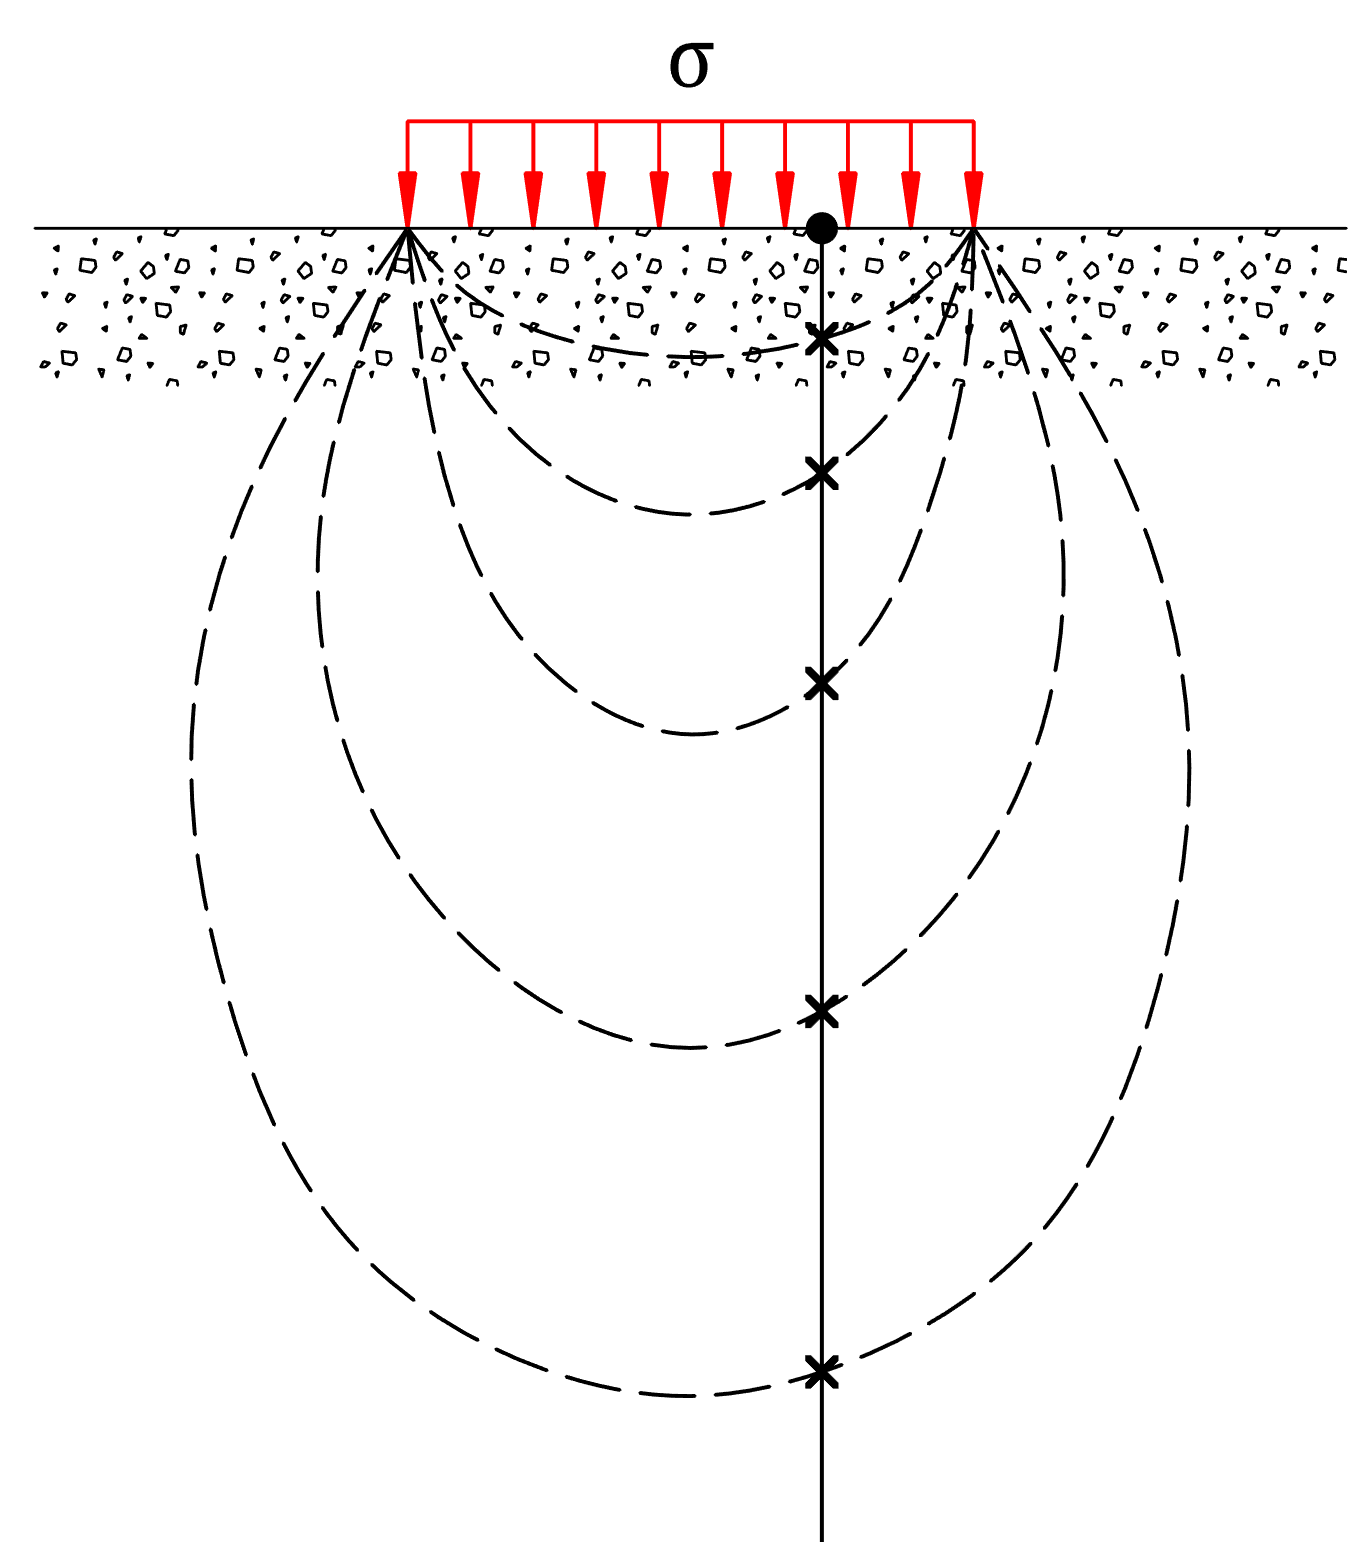
\includegraphics[width=0.5\linewidth,keepaspectratio]{papers/spannung/Grafiken/Bild4.png}
	\caption{Ausbreitung der Zusatzspannung im Boden}
	\label{fig:Bild4}
\end{figure}

\begin{figure}
	\centering
	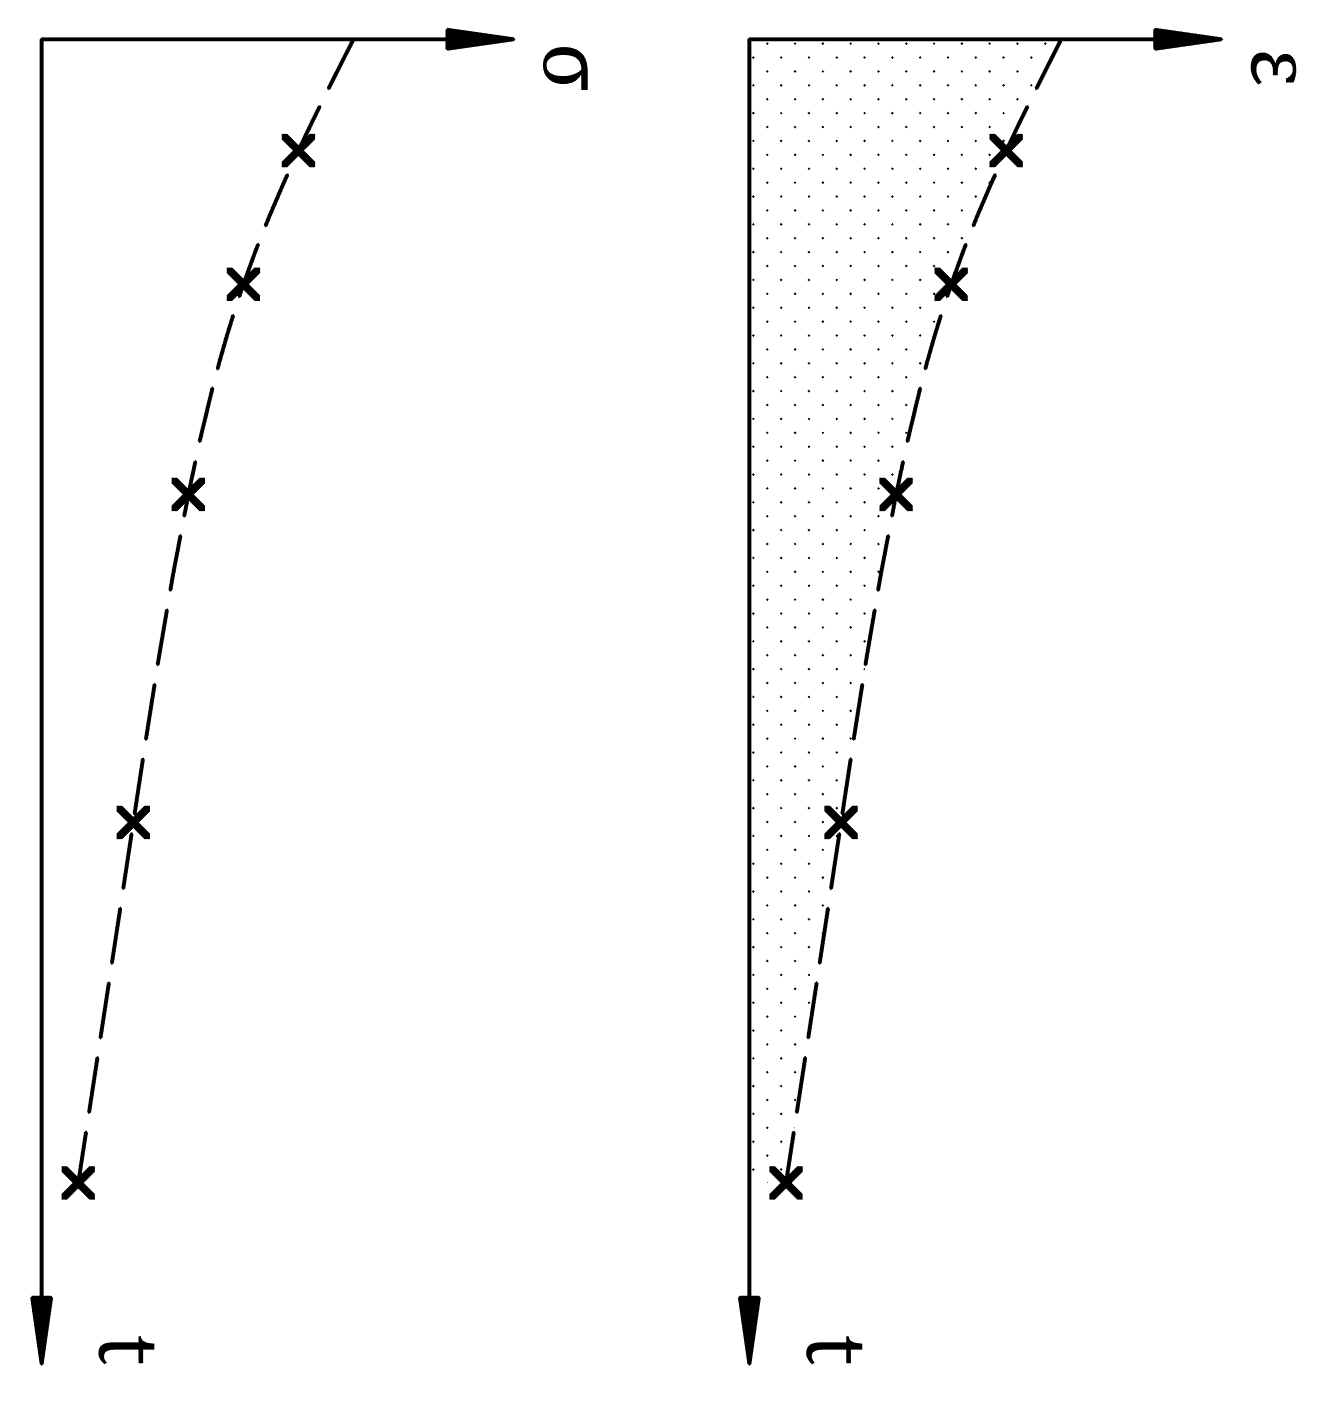
\includegraphics[width=0.5\linewidth,keepaspectratio]{papers/spannung/Grafiken/Bild5.png}
	\caption{Funktionen Spannung und Dehnung}
	\label{fig:Bild5}
\end{figure}

Bei jeder dieser Zusatzspannung geht eine entsprechende Zusatzdehnung einher, welche eine Setzung bedeutet.
Im einfachsten Fall kann modellhaft mit
\[
\varepsilon
=
\frac{\sigma}{E}
\]
die Setzung an einem Punkt an der Bodenoberfläche mit
\[
s
=
\int_{0}^{\infty}\varepsilon\enspace dt
\]
berechnet werden mit:
\[
\varepsilon
=
\text{Dehnung [$-$]}
\]
\[
\sigma
=
\text{Spannung [\si{\kilo\pascal}]}
\]
\[
E
=
\text{Elastizitätsmodul; Young-Modul [\si{\kilo\pascal}]}
\]
\[
t
=
\text{Tiefe [\si{\meter}]}
\]
\[
s
=
\text{Setzung, Absenkung [m]}
\]

In der praktischen Geotechnik wird man allerdings weitaus schwierigere Situationen antreffen.
Ein Beispiel wäre eine Baugrube mit einem Baugrubenabschluss, wo ein Teil des Bodens abgetragen ist (siehe Abbildung 1.3).
Die Ausbreitung der Zusatzspannung $\sigma(x,y,t)$ würde hier deutlich komplizierter ausfallen.
Dies bedeutet auch eine komplexere Setzung der Bodenoberfläche infolge einer Flächenlast $\sigma$.
Aus allen zusätzlichen Spannungen müssen die adäquaten Dehnung mit Hilfe einer Spannungsgleichung berechnet werden.
Diese beruht auf Annahmen nach Hooke auf einem linear elastischen Boden.
Generell wird im Ingenieurwesen versucht Phänomene möglichst nach dem Hook'schen Gesetz abbilden zu können.

\begin{figure}
	\centering
	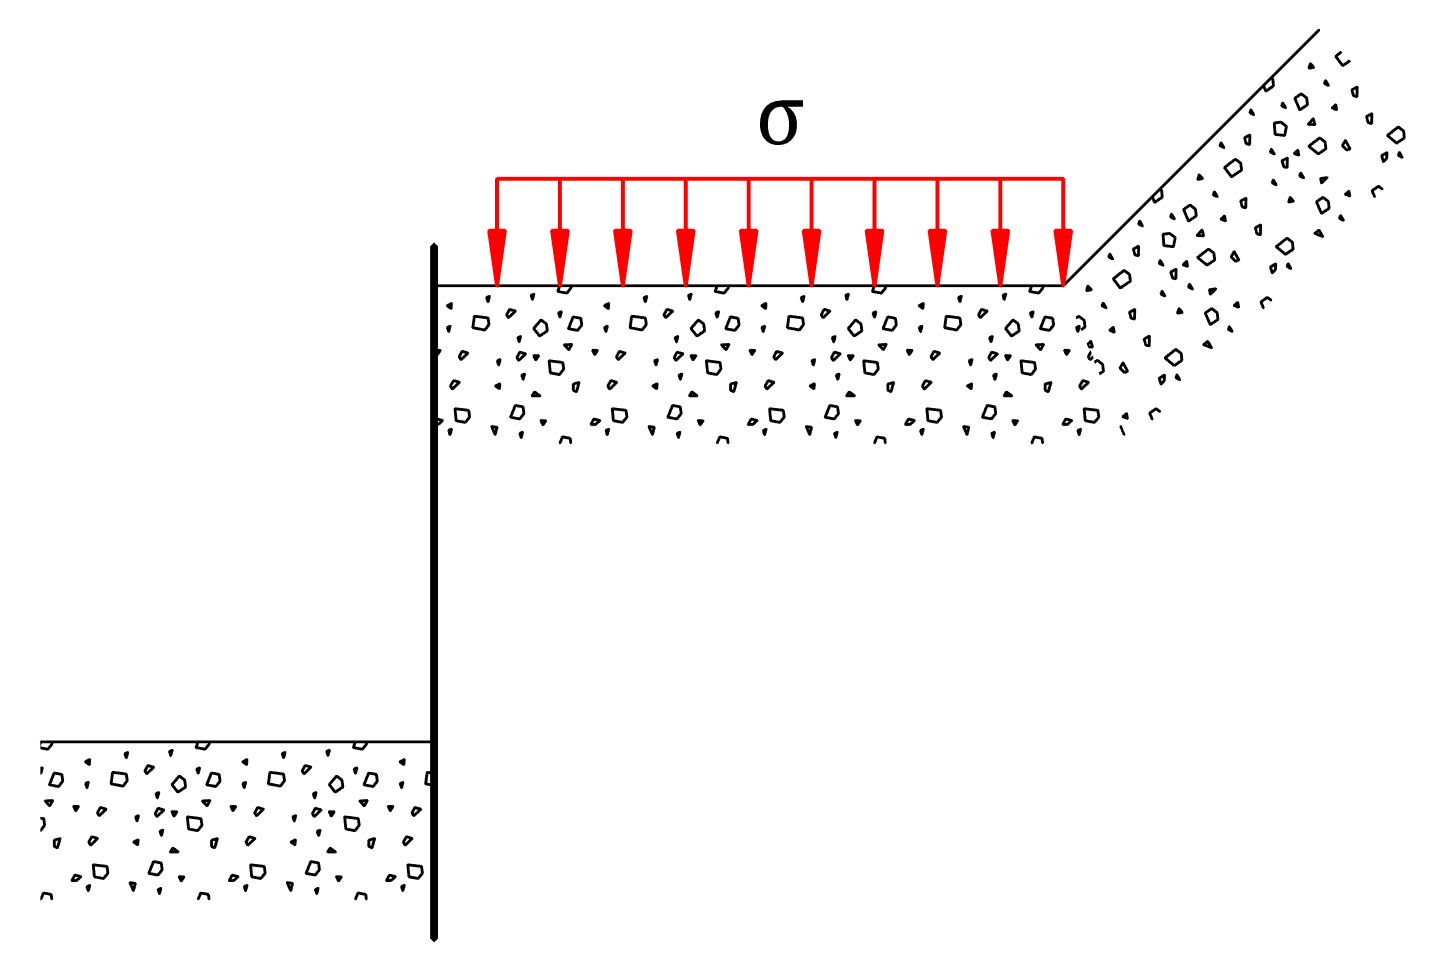
\includegraphics[width=0.5\linewidth,keepaspectratio]{papers/spannung/Grafiken/Bild3.png}
	\caption{Beispiel Lastauftrag auf Boden}
	\label{fig:Bild3}
\end{figure}